\documentclass[12pt]{article}
\usepackage{graphicx}
\usepackage{amsmath}
%\usepackage{float}
%\usepackage{listings}
\setlength\parindent{0pt} % Removes all indentation from paragraphs

\title{Project - Elevator}
\author{Dominik Koszkul, Michal Oleszczyk, Cezary Dynak, Marek Frydrysiak }
\usepackage{geometry}
\newgeometry{tmargin=2cm, bmargin=2cm, lmargin=2cm, rmargin=2cm}
\begin{document}

\maketitle{}
%\tableofcontents{}


\section{Introduction}
The main goal of the project is to develop a controller of a lift system. It will consists of a simulator (depicting a state of a set of lifts) and a controller, which will control their activity basing on users requests and the system state.
\newline \\
The main concept is to create two different programs (one implementing the controller system and the second one for implementation of the elevators simulation). The programs should be independent, i.e. they should use some general protocol for communication, and work failure-free with any other external programs which also use that specified protocol. Both programs start with a set of parameters: a number of elevators and a number of floors supported by any of them. The number of floors does not need to be the same for different elevators. Our elevator controller and simulation do not support underground floors.
\newline
\newline
Assumption: at the very beginning all elevators are in the following state: closed doors on the floor 0 (ground floor). The controller remembers the current state of all the elevators anytime.

\section{Project concept}

\subsection{Module structure}

The module structure of the system is depicted in Figure \ref{fig:DES1}.

\begin{figure}[h!]
  \centering
  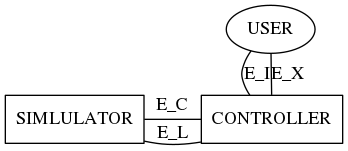
\includegraphics{img/simulator_controller.png}
  \caption{DES graph}
  \label{fig:DES1}
\end{figure}

The system is based on three main parts: the simulator, the controller and the user interface. Essentially, the user interface and the simulator are built within one program. It is as the simulator's part is not only responsible for visualising a state of the lifts, but also it allows a user to interact with it, for instance, by calling a lift on a particular floor choosing a destination floor. 

\subsection{Module communication}

Since the communication protocol between the simulator and the controller is set, it is not necessary for any of them to know how the other works internally. The programs obey the rules of message format, what is sufficiently necessary for a proper communication.
\newline
\newline

The set of events $E$ is described as follows:

\[ E = E^x \cup E^i \cup E^c \cup E^l, \]

where:

\begin{itemize}

\item[]$E^x$ - events from the external buttons,

\item[]$E^i$ - events from the internal buttons,

\item[]$E^c$ - events from the controller,

\item[]$E^l$ - events from the lifts.
\end{itemize}



\section{System model}
\subsection{States}
The state of the system model can be defined as follows:

\[ S = [W, P, Q], \]

where:

\begin{itemize}

\item[]$W$ - lifts state,

\item[]$P$ - external buttons state,

\item[]$Q$ - internal buttons state.

\end{itemize}

The sets of states $W$, $P$, $Q$ are precisely explained in the subsequent sections.

\subsubsection{Lift states}

\[ W=[w_1, w_2, ..., w_i, ..., w_l ],\]
where:
\begin{itemize}
  \item[] \(l\) - number of lifts.
\end{itemize}

For each lift state

\[ w_i = [d_i, o_i, f_i], \]
where:

\begin{itemize}
\item[] \(d \in \{\text{going\_down},\text{stopped},\text{going\_up}\}\),

\item[] \(o \in \{\text{closed},\text{opened}\}\),

\item[] \(f \in \{0,1,...,i,...,n\}\).
\end{itemize}

Moreover

\begin{itemize}
  \item[] \(i\) - next floor to be reached or the current floor,
  \item[] \(n\) - number of floors.
\end{itemize}


\subsubsection{External buttons states}

\[ P = [p_1, p_2, ..., p_i, ..., p_n], \]
where:
\begin{itemize}
  \item[] \(n\) - number of floors,
\end{itemize}

\[ p_i = [g_{i_d}, g_{i_u}], \]
where:\\
\(g_{i_d} \in \{\text{not\_pushed},\text{pushed}\}\),
\(g_{i_u} \in \{\text{not\_pushed},\text{pushed}\}\).\\

Moreover

\begin{itemize}
  \item[] \(d\) - down,
  \item[] \(u\) - up.
\end{itemize}

\subsubsection{Internal buttons states}
\[ Q = [q_1, q_2, ..., q_i, ..., q_l] \]
where:
\begin{itemize}
  \item \(l\) - number of lifts
\end{itemize}
\[q_i = [b_{i_0}, b_{i_1}, ..., b_{i_j}, ..., b_{i_n}] \]
\(b_{i_j} \in \{\text{not\_pushed},\text{pushed}\} \)

\subsection{Events}


\subsubsection{Events from the external buttons} 
\[ E^x = [\text{floor\_nr},\text{direction}] \]

\begin{itemize}
\item[] \(\text{floor\_nr} \in \{0, 1,..., n\}\),
\item[] \(\text{direction} \in \{down, up\}\).
\end{itemize}

\subsubsection{Events from the internal buttons}
\[ E^i = [\text{lift\_nr},\text{button\_nr}] \]
\(\text{button\_nr} \in \{0, 1,..., n\}\)

\subsubsection{Events from the lifts}
\[ E^l = [\text{lift\_nr}, \text{action}] \]
\(\text{action} \in \{\text{going\_down},\text{stopped},\text{going\_up},\text{closed},\text{opened}\}\)

\subsection{Transition functions \(f(s,e)\)}

\subsubsection{Events from the external buttons}
\[
  f(s_0,[\text{lift\_nr},\text{button\_down}]) =
  [0,[[0,0],...,[g_{\text{lift\_nr}_d}=\text{pushed},0],...,[0,0]],0]
\]
\[
  f(s_0,[\text{lift\_nr},\text{button\_up}]) =
  [0,[[0,0],...,[0,g_{\text{lift\_nr}_u}=\text{pushed},0],...,[0,0]],0]
\]


\subsubsection{Events from the internal buttons}
\[
  f(s_0,[\text{lift\_nr},\text{button\_nr}]) =
  [0,[[0,...,0],...,[0,...,b_{\text{lift\_nr}_\text{button\_nr}}=\text{pushed},..,0],...,[0,...,0]],0]
\]


\subsection{Initial state \(s_0\)}
All 0.
\[
  s_0 = [0,0,0]
\]


%\section{Automaton description}

%\[ G = (E, S, f, \Gamma, s_0, S_M) \]

\subsection{Marked states \(S_M\)}
All permitted.

\section{Controller model}

\subsection{Events}
\subsubsection{Events from controller}
\[ E^c = [\text{lift\_nr}, \text{command}] \]
\(\text{command} \in \{\text{go\_down},\text{stop},\text{go\_up},\text{close\_door},\text{open\_door}\}\)

\subsection{Transition function\(f(s,e)\)}



\subsubsection{Events from controller}
\(
  f(s_0,[\text{lift\_nr},\text{go\_down}] =
  [[...,[d_\text{lift\_nr}=\text{going\_down},0,f_\text{lift\_nr}+1],...],0,0]
\)\\
\(
  f(s_0,[\text{lift\_nr},\text{stop}] =
  [[...,[d_\text{lift\_nr}=\text{stopped},0,0],...],0,0]
\)\\
\(
  f(s_0,[\text{lift\_nr},\text{go\_up}] =
  [[...,[d_\text{lift\_nr}=\text{going\_up},0,f_\text{lift\_nr}-1],...],0,0]
\)\\
\(
  f(s_0,[\text{lift\_nr},\text{close\_door}] =
  [[...,[0,o_\text{lift\_nr}=\text{closed},0],...],0,0]
\)\\
\(
  f(s_0,[\text{lift\_nr},\text{open\_door}] =
  [[...,[0,o_\text{lift\_nr}=\text{opened},0],...],0,0]
\)



%\subsection{Active event function \(\Gamma(s)\)}
%Active event function \(\Gamma(s)\) corresponde to tansition function\(f(s,e)\).


\section{Implementation}
\subsection{Simulation}
The simulation program was written in the Python2.7 scripting language. For preparation of the user interface we used the $Tkinter$ standard library. 
The simulation consists of 3 modules: graphics.py, elevator.py and my{\_}threads.py. It implements 2 basic classes:  
\begin{itemize}
 \item Stage - class responsible for drawing the user interface in general (makes windows, buttons, digital panels).
 \item Elevator - class responsible for handling the elevator object (sets its parameters, states). 
\end{itemize}
and classes inheriting from the class $Thread$:
\begin{itemize}
 \item MoveLiftDown - class executes a command type $X:Y$.
 \item StopLift - class executes a command type $X:s$.
 \item MoveLiftUp - class executes a command type $X:Y$.
 \item OpenDoors - class executes a command type $X:o$.
 \item CloseDoors - class executes a command type $X:c$.
 \item ListenInstructions - class listen whether on the input port there is any incoming command or not.
 \item SendInstructions - class sends to the output port a command for controller.
\end{itemize}


The program is basing on 4 main threads (to quarantee the simultaneous work): 
\begin{itemize}
	\item Main thread - is responsible for the parameters configuration, start other thread and waiting for them to finish.
	\item Graphical thread - is responsible for refreshing the user interface (drawing the elevators and the floors) and for sending. 
	\item Listenning thread - is responsible for listening on the input port and adding the incoming instructions to the input queue.
	\item Sending thread - is responsible for sending a command to the controller via the output port if there is an instruction ready to be sent to the output queue.		
\end{itemize}

Furthermore, any command read from the controller (like MoveLift, StopLift, OpenDoor, CloseDoor) takes some predefined time. That is why any of that incoming commands starts another independent thread. In that thread, the commands are executed (for example during the MoveLift command the user interface shows direction of movement, highlighting a specified floor to green). After the execution that thread puts in the output queue a confirmation of the execution for the controller ($X:a$).
	\begin{figure}
	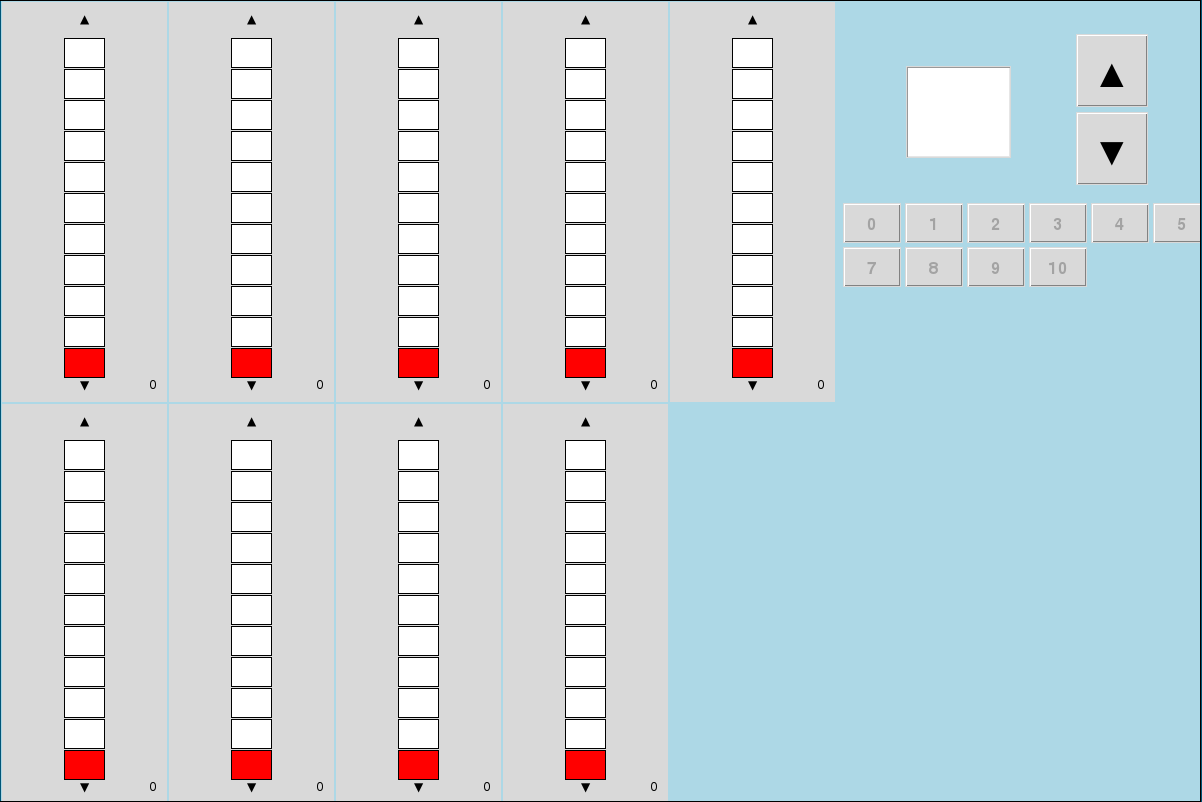
\includegraphics[width=0.93\textwidth]{img/winda.png}
	\end{figure}

\subsection{Controller}

The controller uses the same set of data, as the simulator provides. The exemplary controller execution is listed below

\begin{verbatim}
>> node socket_control.js
floor list: 10,10,10,10,10,10,10,10,10,7,8,20
max floor: 20
W = 
[ [ 0, 0, 0 ],
  [ 0, 0, 0 ],
  [ 0, 0, 0 ],
  [ 0, 0, 0 ],
  [ 0, 0, 0 ],
  [ 0, 0, 0 ],
  [ 0, 0, 0 ],
  [ 0, 0, 0 ],
  [ 0, 0, 0 ],
  [ 0, 0, 0 ],
  [ 0, 0, 0 ],
  [ 0, 0, 0 ] ]
P = 
[ [ 0, 0 ],
  [ 0, 0 ],
  [ 0, 0 ],
  [ 0, 0 ],
  [ 0, 0 ],
  [ 0, 0 ],
  [ 0, 0 ],
  [ 0, 0 ],
  [ 0, 0 ],
  [ 0, 0 ],
  [ 0, 0 ],
  [ 0, 0 ],
  [ 0, 0 ],
  [ 0, 0 ],
  [ 0, 0 ],
  [ 0, 0 ],
  [ 0, 0 ],
  [ 0, 0 ],
  [ 0, 0 ],
  [ 0, 0 ] ]
Q = 
[ [ 0, 0, 0, 0, 0, 0, 0, 0, 0, 0 ],
  [ 0, 0, 0, 0, 0, 0, 0, 0, 0, 0 ],
  [ 0, 0, 0, 0, 0, 0, 0, 0, 0, 0 ],
  [ 0, 0, 0, 0, 0, 0, 0, 0, 0, 0 ],
  [ 0, 0, 0, 0, 0, 0, 0, 0, 0, 0 ],
  [ 0, 0, 0, 0, 0, 0, 0, 0, 0, 0 ],
  [ 0, 0, 0, 0, 0, 0, 0, 0, 0, 0 ],
  [ 0, 0, 0, 0, 0, 0, 0, 0, 0, 0 ],
  [ 0, 0, 0, 0, 0, 0, 0, 0, 0, 0 ],
  [ 0, 0, 0, 0, 0, 0, 0 ],
  [ 0, 0, 0, 0, 0, 0, 0, 0 ],
  [ 0, 0, 0, 0, 0, 0, 0, 0, 0, 0, 0, 0, 0, 0, 0, 0, 0, 0, 0, 0 ] ]
\end{verbatim}


\subsection{Connection}
The connection is based on sockets. The 'incoming' port for the controller is at the same time the 'outup' port for the simulation program and vice versa.
\newline
\newline
For now:
\newline
controller -\textgreater simulation is realised on port 8089,
\newline
simulation -\textgreater controller is realised on port 8090.

\newpage

\subsection{Protocol}
The protocol corresponds to the events defined in the previous section.

\subsubsection{Controller \(\to\) Simulation commands}
\begin{enumerate}
	\item $X:Y$ (where X is the number of an elevator, Y is number of a floor) - let the elevator X move to the floor Y.
	\item $X:s$ (where X is the number of an elevator) - let the elevator X stops.
	\item $X:o$ (where X is the number of an elevator) - let the elevator X opens the door.
	\item $X:c$ (where X is the number of an elevator) - let the elevator X closes the door
\end{enumerate}


\subsubsection{Simulation \(\to\) Controller commands}
\begin{enumerate}
	\item $X:a$ (where X is the number of an elevator) - the elevator X confirms execution of the previous controller command.
	\item $Y:d$ (where Y is the number of a floor) - on the floor Y$^{th}$ user pushes the button to go down.
	\item $Y:u$ (where Y is the number of a floor) - on the floor Y$^{th}$ user pushes the button to go up.
	\item $X:Y$ (where X is the number of an elevator, Y is the number of a floor) - inside the elevator X user pushes the button to go to the Y$^{th}$ floor.
\end{enumerate}	

Command $X:a$ should be send from the simulation to the controller after execution of any controller command. It provides a synchronization between both programs.

\section{Effort}
The task was divided among the group members in the following order:
\begin{enumerate}
\item Michal Oleszczyk - simulation part, documentation
\item Dominik Koszkul - simulation part, documentation
\item Cezary Dynak - controller part, documentation
\item Marek Frydrysiak - controller part, documentation
\end{enumerate}

\end{document}
